\documentclass{article}
\usepackage[utf8]{inputenc}

\title{Materials and Designs for Drones and Ornithopters}
\author{Aakash \\ Email: \href{mailto:me16b001@iittp.ac.in}{me16b001@iittp.ac.in}}
\date{March 2019}
 \usepackage{hyperref}
\usepackage{natbib}
\usepackage{graphicx}

\begin{document}

\maketitle

\section{Introduction}
In recent years, the use of Unmanned Aerial Vehicles(UAV) is playing important roles in different applications. Commonly known as a drone, a UAV is an aircraft that can perform flight missions autonomously without a human pilot onboard, or can be tele-operated by a pilot from a ground station. It is used in many aspects of military and civil broadly, such as aerial photogrammetry, agriculture, warzone, surveillance, traffic and climate monitoring and so on. These stealth crafts are becoming increasingly popular, not just for war and military purposes, but also for everything from wildlife and atmospheric research to disaster relief and sports photography. Drones are becoming the eyes and ears of scientists by surveying the ground for archaeological sites, signs of illegal hunting and crop damage, and even zipping inside hurricanes to study the wild storms. 
 Unmanned aerial vehicle (UAV) research and development has been growing rapidly ever since over the past decade. One of the important aspect in the design of the drones is the selection of the right material, the material has to be strong enough to provide it rigidity and should be aerodynamic and light weight at the same time for longer and efficient time of flight.  

A flapping-wing UAV, also known as ornithopter, usually is about a hand size although the size may vary a lot, it generates required lifting and forward force by flapping its wings. The aerodynamic modelling and simulation of the ornithopter is much more involved \citep{peterson}. This requires knowledge from different domains such as fluid mechanics, material science, electrical engineering and ofcourse computer science.

In the beginning sections we provide an overview of the advancements in design and material selection for the drones or UAVs. Later section follow the overview of the much recent advancement i.e. the ornithopters, although there have been some successful models still this area is under research and development. In the final section we provide the conclusions.

\section{Designing of Drones}
The two most common types of drones are shown in Figure ~\ref{fig:drone} and ~\ref{fig:drone2}, Figure ~\ref{fig:drone} shows the fixed wing drone with rotors for providing lift while Figure ~\ref{fig:drone2} shows a fixed wing type drone.
.UAV design and advancement is a global activity, and an very active area of research.  As we get more and more advanced methods - computer vision, ML and AI to name a few, these machines are getting more and more advanced and acurate in their tasks. In this paper however we will only be covering the mechanical design aspects. 
It is important to make the body and the supporting structures as light as possible, therefore the lightest, and most cost effective materials available are to be considered. One of the most popular types of materials are the composites and fiber reinforced materials. 
\begin{figure}
    \centering
    \begin{minipage}{0.45\textwidth}
        \centering
        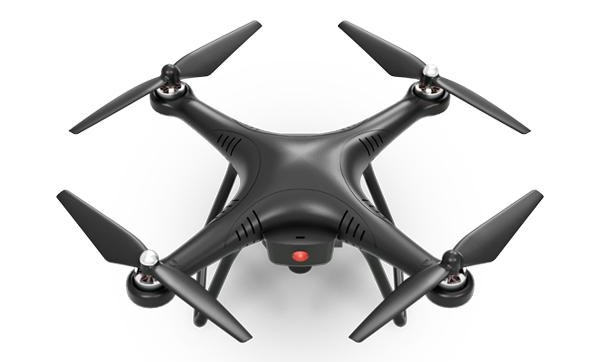
\includegraphics[width=0.9\textwidth]{drone.jpg} % first figure itself
        \caption{Common drone}
        \label{fig:drone}
    \end{minipage}\hfill
    \begin{minipage}{0.45\textwidth}
        \centering
        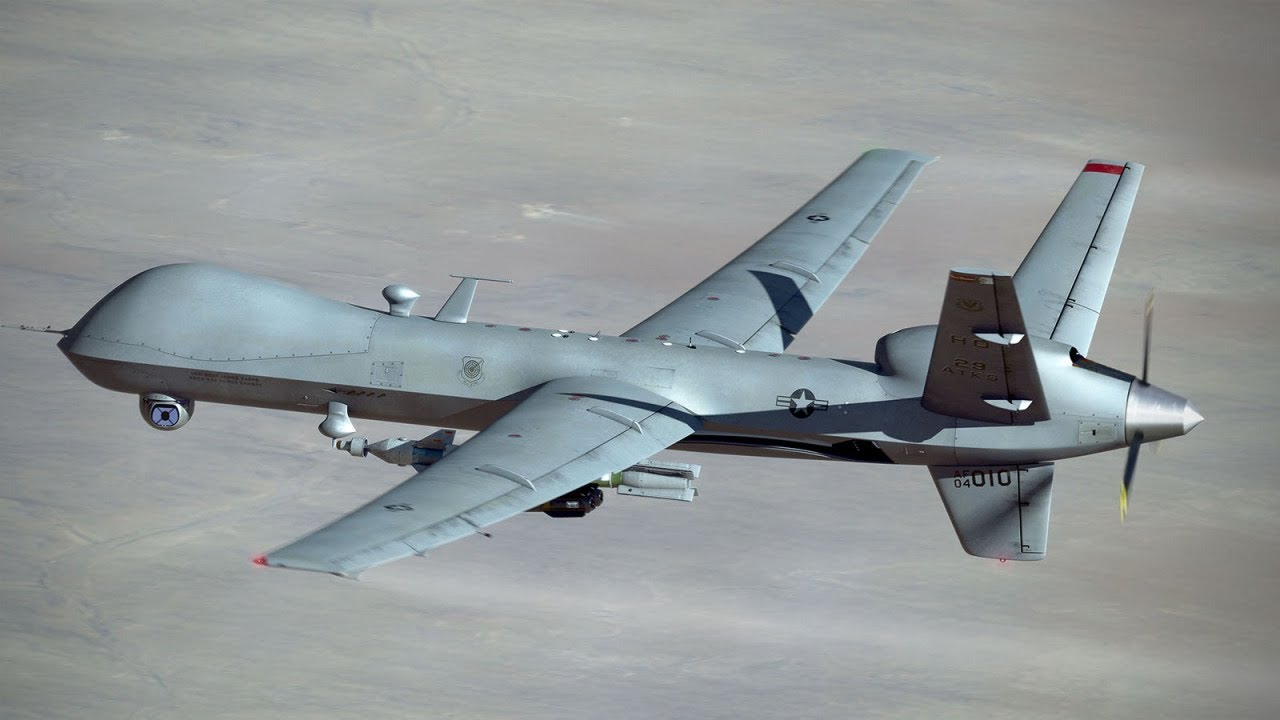
\includegraphics[width=0.9\textwidth]{drone2.jpg} % second figure itself
        \caption{Military drone}
        \label{fig:drone2}
    \end{minipage}
\end{figure}
\subsection{Composite materials}
Due to high requirements of the modern UAV’s (high strength-low weight) composite materials
especially polymer matrix composites reinforced with conti-nues fibers are most appropriate choice \citep{kassapoglou}. The fibres help the material bind better and result in a stronger material do to reinforcement, the fibres also help in taking the tensile loads wherever applicable
These materials are characterized by Young's module twice as high compared to aluminum alloys
while retaining two times lower weight. The difficulties in use of composites materials are related to the anisotropic or orthotropic structure. Performing numerical analysis and simulations for these materials requires sound knowledge of material constants and mechanical properties in principal axes. Only fully defined composite material guarantees real structure behavior and reliability of calculation results \citep{chung}

Composite materials generally consist of two or more phases with significantly different properties, both physical and chemical. Combined together they form a material with characteristics different from individual components. Each phase remain separate within the finished structure. Based on the function played the components of composites can be divided into filler (reinforcement) and matrix. Mostly used matrices materials are polymers, metals, ceramics and carbon while fillers materials are glass, carbon, aramid and boron. Reinforcement occur in different forms: continues fibers, short fibers and particles.

One of the most common composites are the polymer matrix composites. They provide good properties such as low density, high strength, high stiffness, corrosion resistance and vibration damping ability and have low costs fabrication techniques. The most common materials used for matrices are vinyl ester, epoxy, phenol, formaldehyde (PF), polyamide (PI) polyimide and polypropylene (PP) resins. Fillers due to the form of occurrence may take the form of mats (made
form short fibers) or fabrics (continue fibers). The most frequent occurring types of fabrics used as reinforcement for polymer composites are: plain weave, twill wave, satin weave and unidirectional fabric. \citep{krolikowski}.

Another type of composite is the polymer matrix composites, it commonly occurs in form of symmetrical and asymmetrical laminates. Laminates are assemblies of fibrous composites layers, bonded together to provide required engineering properties including strength, stiffness, weight etc. Change in laminate layers orientation significantly affect its properties. 

\begin{figure}[h!]
\centering
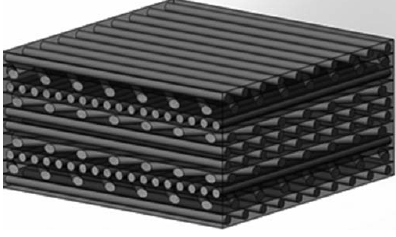
\includegraphics[scale=0.5]{dfm2}
\caption{ Composite laminate with different layer orientations}
\label{fig:universe}
\end{figure}
\subsection{Design of static wing for drones}
Designing of the wings is undoublty the most critical task while designing a fixed wing drone, the properties such as airfoil shape, thickness, chords dimensions, span, surface area and geometry of the wings vary across the length.

It is important to have knowledge about different types of loads acting on designed element while designing the same and selecting materials for the same. In case of design process for UAV wing structures most important loads that are acting on the structure are bending loads and torsion loads derived from acting lift force. Due to high requirements of the modern UAV’s (high strength-low weight) composite materials especially polymer matrix composites reinforced with continues fibers are most appropriate choice. The wing geometry design can be carried out in XFLR 5 software. We are required to carry out detailed numerical simulation of the wing for load and temperature changes it may have to undergo during its flight.

\begin{figure}[h!]
\centering
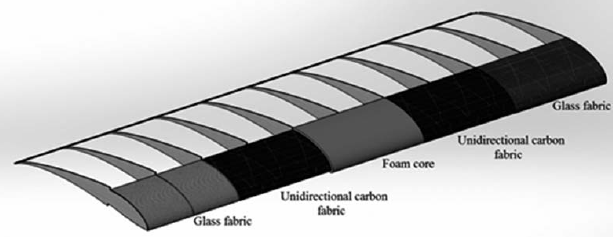
\includegraphics[scale=0.5]{dfm3}
\caption{ Structural design of UAV wing}
\label{fig:universe}
\end{figure}

\section{Designing of Ornithopters}
ToBeDone
\begin{figure}[h!]
\centering
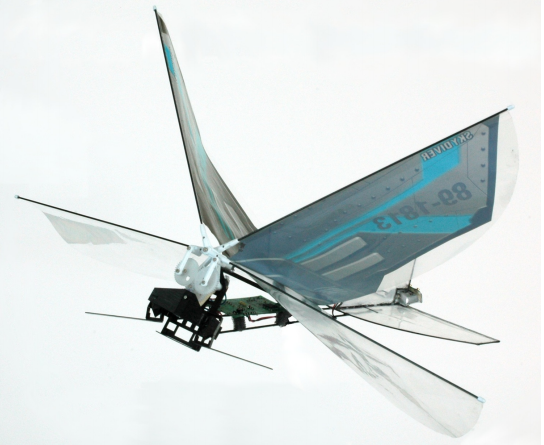
\includegraphics[scale=0.3]{dfm1}
\caption{Ornithopter (courtesy-Peterson et al)}
\label{fig:universe}
\end{figure}

\subsection{Design of flapping mechanisms}
ToBeDone

\subsection{Materials}
ToBeDone

\section{Conclusion}
Designing and developing a UAV is a multistage task which requires many iterations and stages. A typical wing designing process consists of airfoil selection, geometrical calculations, structural design, materials selection, numerical analysis and elaboration of technology. Composite materials prove to be very promising beacuse of their superior properties and light weight, amongst them polymer matrix composites are widely used inaviation industry characterize by high strength-to-weight and stiffness-to-weight ratio \citep{Grodzki}. But as the applications of drones are spreading different domains there is a need to look for more and more materials with extreme properties, for examples scientists have been using drones for studying and examining volcanic activities, here it becomes important to choose the materials wisely which have high temperature resistance.

ToBeDone



\bibliographystyle{plain}
\bibliography{references}
\end{document}
